\documentclass[11pt]{article}

% set these commands
\newcommand{\course}{CSCI 534}
\newcommand{\proj}{Homework 05}
\newcommand{\dueDate}{3-25-2021}
\newcommand{\instructor}{David L. Millman}

\usepackage{macros}

\begin{document}

{ ~\\
    \course \\ 
    \proj \\ 
    Due \dueDate \\
    \instructor
}

\section*{Problem 1 (10 points)}

In Homework 1, we considered a plane-sweep algorithm for determining whether
there is any intersection among a collection of $n$ circles in the plane. Here
we consider a variant of this problem. The input consists of a collection of $n$
closed circular disks, all having the same radius. (Via scaling, we may assume
that they are all unit disks.) Let $C = \{c_1, \ldots , c_n\}$ denote the center
points of these disks, and let $\{D_1, \ldots, D_n\}$ denote the actual disks.
Thus, $D_i$ consists of the points that lie within unit distance of $c_i$. Let
$U = D_1 \cup \ldots \cup D_n$ denote the union of these disks. The boundary of
$U$ may generally consist of multiple parts, each of which consists of a cycle
of circular arcs connected by vertices. (In Fig. 4 the boundary consists of
three cycles. The vertices are shown as white dots).

\begin{figure}[h]
    \centering
    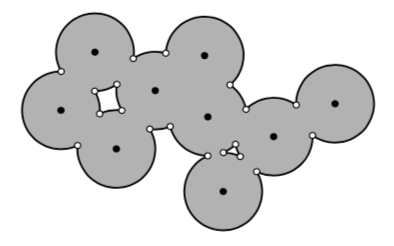
\includegraphics[width=0.4\textwidth]{union-of-disks}
    \caption{Problem 4: Union of disks}
\end{figure}


\begin{enumerate}

    \item Present an algorithm that reports all the vertices on the boundary of
        $U$. (Note that circle intersection points in the interior of the union
        are explicitly excluded.) Your algorithm should run in time $O(n log
        n)$.  The order in which the vertices are output is arbitrary. (Hint:
        Don't try to modify the algorithm from Homework 2. A different approach
        is needed.... think giraffes)

    \item Prove that the number of vertices reported by your algorithm is
        $O(n)$.

\end{enumerate}


\section*{Problem 2 (5 points)}

Suppose we are given a subdivision of the plane into $n$ convex regions. We
suspect that this subdivision is a Voronoi diagram, but we do not know the
sites. Develop an algorithm that finds a set of $n$ point sites whose Voronoi
diagram is exactly the given subdivision, if such a set exists.


\section*{Tips and Acknowledgements}

{\bf Acknowledgements:} Homework problems adapted from assignments of David
Mount and Carola Wenk.

\end{document}
